\section{Uso de un intérprete de comandos especial para las prácticas}

En el ámbito informático, una shell o intérprete de comandos es un programa que proporciona una interfaz de usuario para el acceso a los servicios del sistema operativo. Es lo que se ejecuta cuando se abre una consola de comandos o cuando se crea una conexión segura con un servidor remoto a través del protocolo SSH.

Existen multitud de intérpretes de comandos, cada uno con sus características y sintaxis determinada. El más típico en los sistemas Linux es \textbf{bash}, pero también se usan mucho otros como \textbf{zsh} y \textbf{fish}. En estas prácticas utilizaremos un shell llamado \textbf{Xonsh}, que está escrito en Python y presenta múltiples ventajas, entre ellas:

\begin{itemize}
    \item Es un proyecto de código abierto y con una comunidad activa (en la que puedes participar).
    \item Esta escrito en Python, lo que lo hace fácil de entender y de modificar (o añadir extensiones).
    \item Es compatible con la sintaxis de Python pero también con las de bash y zsh por lo que resulta fácil de aprender y de utilizar \cite{tutorial_xonsh}.
    \item Dispone de un historial enriquecido que permite almacenar datos y metadatos de las sesiones  que puede ser modificado fácilmente para añadir funcionalidades (guardar el historial en una base de datos, enviarla a un servidor o detectar ciertos comandos y evitar su ejecución podrían ser algunas ideas).
    \item Cuenta con un prompt muy personalizable y con opciones avanzadas de colores, animaciones, etc...
\end{itemize}

Además, utilizaremos una versión de Xonsh que cuenta con una herramienta llamada Xxh, que permite crear conexiones ssh en las que se envía la imagen 

\subsection{Instrucciones de instalación}

Para simplificar el uso de Xonsh se propone utiliza una imagen portable del software generada utilizando el framework de offsh, un proyecto opensource que permite crear imágenes de shell con software y configuraciones embebidas\footnote{\url{https://github.com/offsh/offsh}}.

Para hacerlo funcionar basta con descargar la imagen portable y hacerla ejecutable usando chmod. Luego, para terminar su configuración tendríamos que descargar los archivos de configuración de xonsh y xxh.

\textbf{nota: se necesita git instalado en el sistema para que el shell funcione correctamente.}


\begin{lstlisting}[language=bash,caption={Install xonsh using offshell appimage}, label=installxonsh]
sudo wget -q https://github.com/offsh/offsh/releases/download/0.0.2/xonsh -O /bin/xonsh
sudo chmod a+x /bin/xonsh

wget -q https://raw.githubusercontent.com/offsh/offshell/main/xonshrc -O ~/.xonshrc
mkdir -p ~/.config/xxh/
wget -q https://raw.githubusercontent.com/offsh/xxh/master/config.xxhc -O ~/.config/xxh/config.xxhc
\end{lstlisting}

\begin{figure}[pbth]
  \centering
  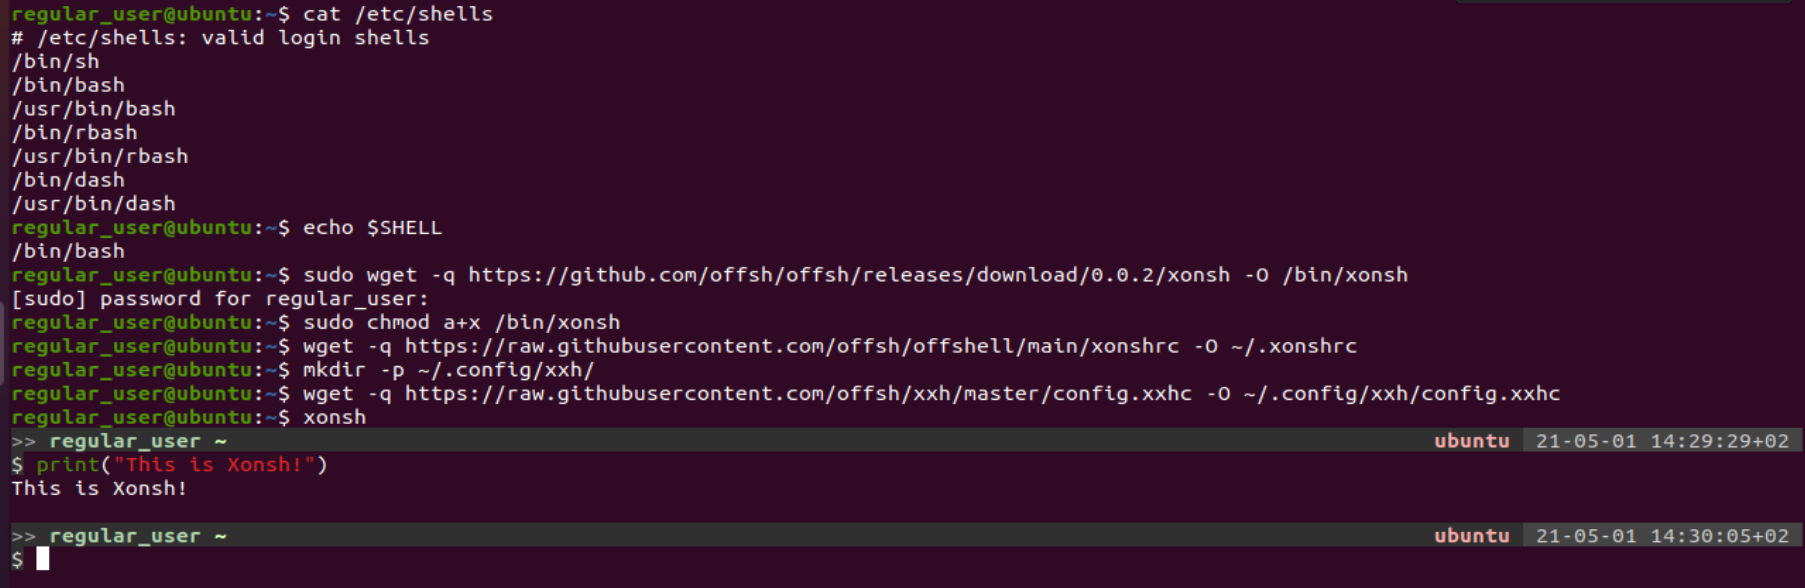
\includegraphics[width=\textwidth]{imagenes/installxonsh.png}
  \caption{En la figura se aprecia como, en un intérprete bash (en una máquina ubuntu similar a las usada en las prácticas), se ejecutan los comandos expuestos en el Listing \cite{installxonsh} para la instalación y configuración de Xonsh. Se puede apreciar como al finalizar de descargar los archivos y ejecutar Xonsh, se dispone de una consola de comandos totalmente diferente a la original (bash).}
  \label{xonsh_install}
\end{figure}

El objetivo de utilizar Xonsh es familiarizarse con el uso de distintos shells (además del que pueda venir por defecto en el sistema) y con la configuración de los mismos. Además, dado que Xonsh tiene un historial enriquecido, podemos generar un fichero con logs como el que se muestra en la figura \ref{xonsh_history}, que servirá para poder llevar un registro de los comandos ejecutados durante las prácticas (con su output, resultado, usuario activo, etc...) y que podrá ser enviado al profesor como parte de la evaluación para comprobar si se han ejecutado correctamente algunos comandos y extraer algunos datos estadísticos (errores más comunes, comandos más ejecutados, tiempo medio de las sesiones, etc...).

\begin{figure}[pbth]
  \centering
  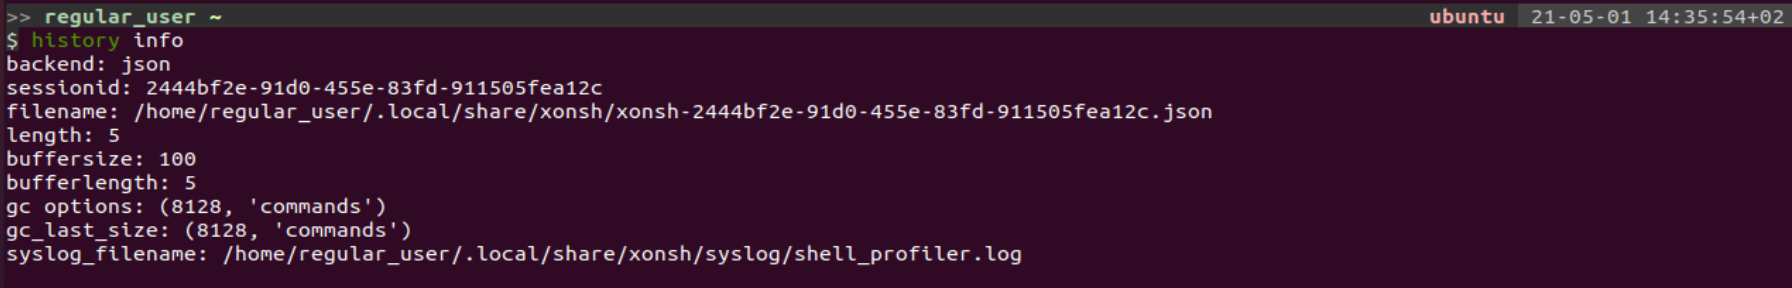
\includegraphics[width=\textwidth]{imagenes/historyinfo.png}
  \caption{Ejemplo de ejecución del comando \textit{history info} en Xonsh, que la información del objeto que contiene el historial de la sesión actual. Existen dos archivos que son referenciados en este comando. Un JSON que contiene todos los datos y metadatos generados por Xonsh por los comandos ejecutados durante esta sesión (efímero, y que se borra cada cierto tiempo) y un fichero `shell\_profiler.log' que tiene formato Syslog y no se borra salvo que se haga manual, y que contiene solo la información que se ha configurado para ser almacenada en offsh.}
  \label{xonsh_history}
\end{figure}

\begin{figure}[phbt]
  \centering
  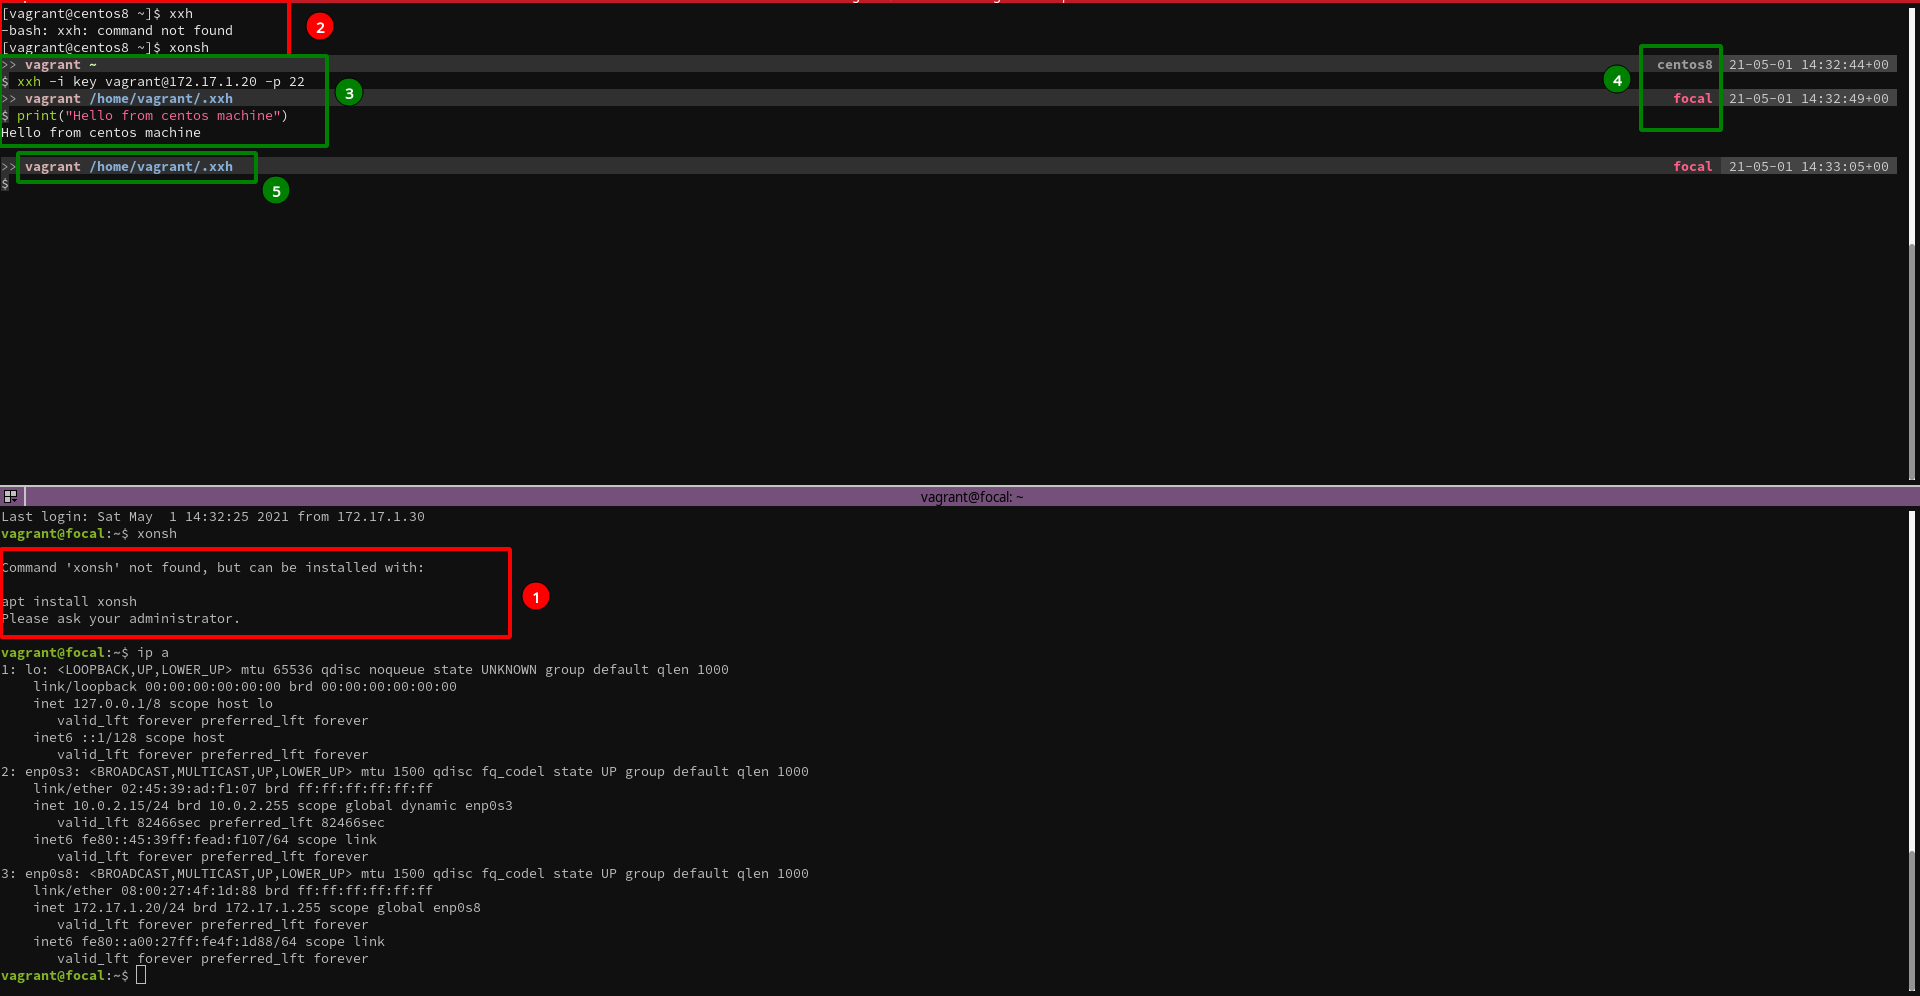
\includegraphics[width=\textwidth]{imagenes/examplexxh.png}
  \caption{En la imagen se muestran dos máquinas virtuales que han sido desplegadas usando el software Vagrant. Una es una máquina centos y la otra, un Ubuntu Focal (1). En Ubuntu Focal se trata de ejecutar Xonsh pero el comando falla, porque este shell no se encuentra instalado en el sistema. Del mismo modo, en Centos se trata de ejecutar Xxh y se produce un error porque el comando tampoco está instalado (2). Al entrar a una sesion de xonsh en la máquina centos, xxh pasa a estar disponible (ya que se encuentra instalado dentro de la imagen de xonsh) y se puede utilizar para conectar por medio de ssh con la máquina focal (3), a la que se enviará la imagen portable de Xonsh, lo que nos permite abrir una sesión de xonsh en la máquina aunque no tenga el software instalado. Es importante notar el cambio de hostname (4) en el prompt de xonsh al cambiar de una máquina a la otra, así como el directorio en el que se crea la sesión (5) que es un directorio temporal creado dentro del directorio home del usuario, oculto, llamado `.xxh'.}
  \label{xxhexample}
\end{figure}

Por último, se propone el uso de Xxh para acceder a las distintas máquinas virtuales desplegadas durante las prácticas utilizando una consola interactiva de xonsh, de forma que podamos familiarizarnos con el uso de distintos shells, así como el uso de ssh y otros sofwares que permitan un mayor control de la sesión utilizando dicho protocolo. Tal y como se muestra en la figura \ref{xxhexample}, en la que se añaden algunas indicaciones sobre el uso de la herramienta.



Finalmente, cabe destacar que al final de una sesión xxh, los logs generados en dicha sesión remota se descargan automáticamente y se integran de forma que se puede mantener un único fichero.

\section{Acuerdo de consentimiento y limitación de la responsabilidad durante el desarrollo de una auditoría de ciberseguridad}\label{acuerdo}

A continuación se propone un ejemplo de texto que podría ser añadido a un contrato de trabajo como auditor de ciberseguridad (o pen-tester) para la autorización por parte de la empresa de las actividades a realizar durante la auditoría, así como la limitación de la responsabilidad de las repercusiones de las mismas.

\textit{Este documento establece que ambas partes comprenden y aceptan el hecho de que existen ciertos riesgos asociados con las actividades que se llevan acabo durante un test de penetración de sistemas, especialmente sobre aquellos sistemas ligados a entornos de producción. }


\textit{El auditor no se hace responsable de ninguna acción (u omisión) que durante la ejecución de las pruebas que en este contrato se han acordado, pueda dañar o dificultar las operaciones de los servicios que se están probando, incluso si las acciones sobrepasan los límites legales. }

\textit{El cliente considera las acciones ligadas a la investigación de vulnerabilidades de sus sistemas consistentes con su política de empresa y autoriza al auditor a llevarlas a cabo dentro del marco legal, incluso aquellas que contradicen leyes como la de acceso no autorizado a los sistemas. En última instancia, es  el cliente el que se responsabiliza de la integridad de su sistema y el auditor solo es responsable de notificar todas aquellas vulnerabilidades y problemas que haya podido encontrar, especialmente si durante las pruebas pertinentes ha detectado algo que pueda causar problemas al cliente.
}